\documentclass[main.tex]{subfiles}

\begin{document}
	\chapter{La topologie quotient}
	Dans tout ce chapitre $X$ dénote un espace \emph{topologique}, $q$ une surjection. Sauf mention du contraire lorsqu'il est question d'espaces topologiques une application est considérée continue.

	\begin{notation}
		Nous introduisons les notations élémentaires qui suivront dans tout le chapitre.
		\begin{list}{$\circ$}{}
			\item Le singleton est l'espace $\star$ il s'agit de l'ensemble à un seul point munit de la topologie discrète. 
			\item L'espace $D^n$ est la boule unité fermée (disque) dans $\mathbf{R}^{n}$ pour la métrique euclidienne usuelle. On notera parfois $e^{n}$ pour ce même espace. L'intérieur $\mathring{D}^n$ ou $\mathring{e}^n$ est donc la boule ouverte. 
			\item Le bord $\partial D^n$ de $D^n$ est la sphère unité $S^{n-1}$. 
			\item On utilise le symbole $\cong$ pour les isomorphismes et les homéomorphismes sans plus de précision tant que le contexte est clair et $\simeq$ pour les homotopies.
			\item Les vecteurs sont notés en gras.
		\end{list}
	\end{notation}

	\section{Théorie générale}
	\begin{definition}[Topologie quotient]
		Étant donné une application $q$, la topologie quotient sur $Y$ relativement à $q$ a pour ouverts les sous ensembles $U \subset Y$ tels que $q^{-1}(U)$ est ouvert dans $X$.
	\end{definition}
	\begin{remark}
		Une caractérisation équivalente de cette topologie peut se faire en définissant les fermés de $Y$ par les fermés de $X$.
	\end{remark}
	\begin{definition}[Quotient]
		On dit qu'une application $q : X \longmapsto Y$ est un quotient si elle est surjective, continue et que la topologie quotient induite par $q$ coïncide avec la topologie de $Y$.	
	\end{definition}
	\begin{prop}
		Si $q : X \longmapsto Y$ est une application surjective continue et ouverte alors $q$ est un quotient et $Y$ est muni de la topologie quotient définie par $q$.
	\end{prop}
	\begin{proof}
		Si $U$ est ouvert dans $Y$ alors $q^{-1}(U)$ est ouvert dans $X$ par continuité de $q$. Réciproquement si  $ U \subset Y$ et $q^{-1}(U)$ est ouvert dans $X$ alors par surjectivité de $q$  \[
			q(q^{-1}(U)) = U
		\] et on en conclut que $U$ est ouvert dans $Y$ puisque $q$ est ouverte. 
	\end{proof}
	\begin{remark}
		Ce critère reste valable si $q$ est une application fermée, la preuve est identique en remplaçant les ouverts par des fermés.
	\end{remark}
	\begin{example}
		Il est cependant important de noter que ce critère bien que suffisant n'est \emph{pas} nécessaire. Définissons l'application\\

		\noindent \begin{minipage}{0.5\textwidth}
		\begin{align*}
			q : [0,3] &\longmapsto [0,2]\\
			t &\longmapsto \begin{cases}
				t \text{\; si \;} t \le 1\\
				1 \text{\; si \;} 1 \le t \le 2\\
				t-1 \text{\; sinon}
			\end{cases}
		.\end{align*}
		\end{minipage}
		\hfill
		\noindent \begin{minipage}{0.5\textwidth}
			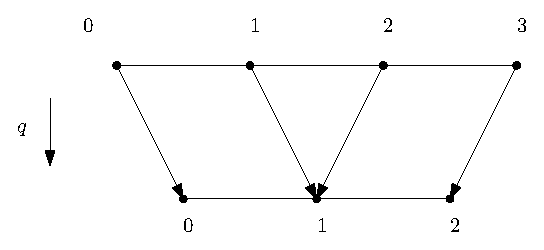
\includegraphics[width=\linewidth]{example_1.eps}
		\end{minipage}\\

		$q$ est une application continue, c'est un quotient pour la topologie euclidienne sur $[0,3], [0,2]$ mais elle n'est pas ouverte,  $(1,2)$ est envoyé sur $\{1\}$.
	\end{example}

	\begin{prop}
		La composition de deux quotients est également un quotient.
	\end{prop}
	\begin{prop}[Propriété universelle]
		\label{prp:1}
		La topologie quotient est la plus fine telle que l'application $q$ soit continue. De plus, $g : Y \longmapsto Z$ est une application continue si et seulement si $g \circ q : X \longmapsto Z$ est continue.
	\end{prop}
	\begin{proof}
		Soit $U$ un ouvert d'une topologie sur $Y$ telle que $q$ soit continue. Par continuité $q^{-1}(U)$ est ouvert dans $X$ et donc $U$ est ouvert dans $Y$ pour la topologie quotient. 
	Si $g$ est continue, $g\circ q$ est continue en tant que composition d'applications continues. Réciproquement, si  $g \circ q$ est continue prenons $V \subset Z$ un ouvert, ${(g\circ q)}^{-1}(V)$ est ouvert dans $X$ par continuité de la composée et de plus \[
			q^{-1}(g^{-1}(V)) = {(g\circ q)}^{-1}(V)
		\] est ouvert. Ainsi par définition de la topologie quotient $g^{-1}(V)$ est ouvert dans $Y$ ce qui conclut quant à la continuité de $g$. 
	\end{proof}

	\begin{example}
		Considérons le cercle unité \[
			C \defeq \{(x,y) \in \mathbf{R}^2 \;|\; x^2 + y^2 = 1\} 
		.\] 
		On définit $q$ une application surjective comme suit \\ 
		\begin{minipage}{0.5\textwidth}
			\begin{align*}
				q : \mathbf{R} &\longmapsto C\\
				t&\longmapsto e^{2\pi it}
			.\end{align*}	
		\end{minipage}
		\hfill
		\begin{minipage}{0.5\textwidth}
			\centering
			\begin{tikzpicture}
				\draw[thick] (0,0) ellipse (2cm and 0.5cm);
				\draw[thick,decoration={aspect=0.31, segment length=7mm,
				amplitude=2cm,coil},decorate,arrows = {<[bend]-}] (0,1) --(0,4);
				\draw[->,thick] (3,3) -- (3,1);
				\node at (3.5,2) {$q$};
				\node at (2.5,4) {$\mathbf{R}$};
				\node at (2.5,0) {$C$};
			\end{tikzpicture}
		\end{minipage}
		\bigskip

		Il s'agit d'une application continue surjective et ouverte pour la topologie euclidienne, c'est donc un quotient.
	\end{example}
	
	\begin{prop}
		Si $q$ est un quotient $X \longmapsto Y$ et que $X$ est compact alors $Y$ est aussi compact.
	\end{prop}
	\begin{proof}
		L'image d'un compact par une fonction continue est un compact.
	\end{proof}

	\section{Quotient par une relation}
	Étant donné une relation d'équivalence $\sim$ on note $[x]$ la classe d'équivalence de  $x \in X$.
	\begin{definition}[Espace quotient]
		On définit une application
		\begin{align*}
			q : X &\longmapsto \quot{X}{\sim} \\
			x &\longmapsto [x]
		\end{align*}
		alors l'espace quotient de $X$ par $\sim$ est l'ensemble $\quot{X}{\sim}$ munit de la topologie quotient induite par $q$.
	\end{definition}
	\begin{remark}
		On peut munir une partition $X^*$ de $X$ de la topologie quotient en définissant une relation d'équivalence $\sim$ sur  $X^*$ comme suit \[
			x \sim y \iff \exists A \in X^* \; \text{tel que} \; x,y \in A
		.\] 
	\end{remark}
	\begin{example}
		Le cercle $C$ définit précédemment peut être vu comme espace quotient de $[0,1]$ par la relation 
		 \begin{align*}
			x \sim y \iff \begin{cases}
				x = y \\
				x,y \in \{0,1\}
			\end{cases}
		.\end{align*}
	\end{example}

	\begin{prop}[Propriété universelle]
		Soit $\sim$ une relation d'équivalence sur un espace $X$, pour toute application $f : X \longmapsto Y$ vérifiant $x \sim x' \implies f(x) = f(x')$ il existe une unique application $\hat{f} : \quot{X}{\sim} \longmapsto Y$ telle que $\hat{f} \circ q = f$. On dit que $f$ \textbf{passe au quotient} et induit une application $\hat{f}$. \\
		\begin{minipage}{0.5\textwidth}
			Le diagramme suivant résume cette propriété, $\hat{f}$ est l'unique fonction le faisant commuter.
		\end{minipage}
		\hfill
		\begin{minipage}{0.5\textwidth}
			\centering
			\begin{tikzcd}[row sep=large]
				X \arrow[r, "q"] \arrow[dr, "f"]
		    & \quot{X}{\sim} \arrow[d, dashed, "\exists! \; \hat{f}"]\\
		&D
			\end{tikzcd}
		\end{minipage}
	\end{prop}
	\begin{proof}
		Comme on veut $\hat{f}\circ q = f$ on doit avoir $\hat{f}([x]) = \hat{f}(q(x)) = f(x)$ et l'unicité est garantie. Cette application est bien définie puisqu'on a imposé que $f$ soit compatible avec $\sim$. Pour vérifier la continuité de $\hat{f}$ il suffit de réaliser que la composition $\hat{f} \circ q$ est continue puisqu'il s'agit de $f$ et d'appliquer la \textbf{Proposition} \ref{prp:1}. 

	\end{proof}
	Soit $A\subset X$ un sous espace.
	\begin{definition}[Collapse]
		Le collapse de $X$ par $A$ est le quotient $\quot{X}{\sim}$ où
		 \begin{align*}
			x \sim x' \iff \begin{cases}
				x=x' \\
				x,x' \in A
			\end{cases}
		.\end{align*}
		On le note $\quot{X}{A}$.
	\end{definition}
	\begin{example}
		Le cercle unité définit précédemment s'écrit comme le collapse $C = \quot{[0,1]}{\{0,1\}}$.
	\end{example}

	\begin{example}
		On cherche à montrer ici que le collapse $\quot{D^n}{S^{n-1}}$ est homéomorphe à la sphère unité $S^n$. Le cas $n=2$ est très visuel.
		\begin{figure}[ht!]
			\centering
			\incfig{dessin}
			\caption{Illustration de ce quotient dans le cas $n=2$.}
		\end{figure}
		On exhibe à présent l'homéomorphisme dans le cas général
		\begin{align*}
			f : D^n &\longmapsto S^n \\
			\textbf{x} &\longmapsto \begin{cases}
				(2\textbf{x},\sqrt{1-\|\textbf{2x}\|^2}) \; &\text{si} \; \|\textbf{x}\| \le \frac{1}{2} \\
				([4-4\|\textbf{x}\|]\textbf{x},-\sqrt{1-{[4-4\|\textbf{x}\|]}^2{\|\textbf{x}\|}^2}) \; &\text{si} \; \frac{1}{2} \le \|\textbf{x}\| \le 1
			\end{cases}
		.\end{align*}
		Tout point du bord de $D^n$, donc de norme 1, est envoyé sur  $(\textbf{0},-1)$, cette application passe donc au quotient et induit une application $\hat{f} : \quot{D^n}{S^{n-1}} \longmapsto S^n$. Puisque c'est une bijection continue d'un espace compact vers un espace séparé il s'agit d'un homéomorphisme.
	\end{example}

	\begin{definition}[Union disjointe]
		Étant donné une famille d'ensembles $\{X_i \;|\; i \in I\}$ indexés par un ensemble d'indices $I$, l'union disjointe est l'ensemble \[
			\coprod_{i \in I}X_i \defeq \bigcup_{i\in I}\{(x,i) \;|\; x\in X_i\} 
		.\]
		On définit une topologie sur cet ensemble telle que les inclusions canoniques 
		\begin{align*}
			\varphi_i : X_i &\longmapsto \coprod X_i \\
			x&\longmapsto(x,i)
		\end{align*} soient continues. De façon explicite un sous ensemble $U \subset \coprod X_i$ est ouvert si et seulement si sa préimage $\varphi_{i}^{-1}(U) \subset X_i$ est ouverte pour tout $i\in I$. Cette topologie est appelée topologie coproduit.
	\end{definition}
	\begin{prop}[Propriété universelle]
		L'union disjointe d'une famille d'ensembles munie des injections canoniques est caractérisée par la propriété universelle suivante. \\

		\begin{minipage}{0.5\textwidth}
			Pour tout espace $Y$ et toute application continue $f_i : X_i \longmapsto Y$ pour $i \in I$, il existe une unique application continue \[f : \coprod X_i \longmapsto Y\] telle que $f \circ \varphi_i = f_i$. Cette propriété est résumée par le diagramme suivant.	
		\end{minipage}
		\hfill
		\begin{minipage}{0.5\textwidth}
			\centering
			\begin{tikzcd}[row sep=huge]
				X_i \arrow[r, "\varphi_i"] \arrow[dr, "f_i"]
		    & \coprod X_i \arrow[d, dashed, "\exists! \; f"]\\
		&Y
			\end{tikzcd}
		\end{minipage}
	\end{prop}

	\bigskip
	\begin{prop}
		La topologie coproduit est la moins fine telle que les projections canoniques soient continues.
	\end{prop}

	\begin{definition}[Wedge]
		Si $(X_i,x_i)$ est un espace épointé pour $i\in I$ un ensemble d'indices non vide, alors le wedge ou \emph{bouquet} en français, noté $\bigvee_{i\in I} X_i$, est le quotient de l'union disjointe des $X_i$ par la relation
		 \begin{align*}
			x\sim x' \iff \begin{cases}
				x=x' \\
				x,x' \in \{x_i \;|\; i\in I\} 
			\end{cases}
		.\end{align*} 
	\end{definition}
	\begin{example}
		Le wedge $S^1 \bigvee S^1$ est un huit, par abus de notation on admet de mentionner le point de base lorsque le choix de ce dernier n'a pas d'importance.
	\end{example}

	\begin{definition}[Cylindre et cône de base $X$]
		Pour un espace $X$, le cylindre de base $X$ est $X \times I$ avec le plus souvent $I = [0,1]$.
		Le cône de base $X$ est le quotient $\quot{X\times I}{X \times 0}$, on le note $CX$.
	\end{definition}

	\begin{figure}[!ht]
	    \centering
	    \incfig{dessin2}
	    \caption{Illustration du cylindre et du cône de base $X$.}
	\end{figure}

	\begin{definition}[Suspension]
		La suspension d'un espace $X$ s'obtient à partir du cylindre $X \times I$ en collapsant $X \times 0$ ce qui donne le cône de base $X$ puis en collapsant $X \times 1$. On la note \[
			\Sigma X \defeq \quot{CX}{X \times 1}
		.\] 	
	\end{definition}

	\begin{definition}[Homotopie]
		Deux fonctions $f,g : X \longmapsto Y$ sont dites homotopes et on note $f \simeq g$ s'il existe une application $H : X \times I \longmapsto Y$ telle que pour tout $x$ dans $X$ 
		\begin{align*}
			H(x,0) = f(x) \\
			H(x,1) = g(x)
		.\end{align*} On dit alors que $H$ est une homotopie de $f$ vers $g$.
	\end{definition}

	\begin{definition}[Type d'homotopie]
		On dit que deux espaces $X$ et $Y$ ont le même type d'homotopie s'il existe des applications $f : X \longmapsto Y$ et $g : Y \longmapsto X$ telles que $f \circ g \simeq id_Y$ et $g \circ f \simeq id_X$. On note alors $X \simeq Y$ et on appelle $f$ et $g$ des équivalences d'homotopie.	
	\end{definition}

	\begin{prop}
		Le cône $CX$ est toujours contractile, c'est à dire qu'il a le même type d'homotopie qu'un singleton.	
	\end{prop}
	\begin{proof}
		On définit 
		\begin{align*}
			H : X \times I \times I &\longmapsto X \times I \\
			(x,s,t) &\longmapsto (x,st)
		.\end{align*}
		Cette application est clairement continue, elle passe au quotient et induit une application
		\begin{align*}
			\overline{H} : CX \times I &\longmapsto CX \\
			([x,s],t) &\longmapsto [x,st]
		.\end{align*}
		Cette dernière application est bien définie puisque $H(x,0,t) = (x,0)$. Cette application  $\overline{H}$ est une homotopie entre $\overline{H} \vert_{CX \times 0}$
		qui est l'application constante sur $[x,0]$ et $\overline{H} \vert _{CX \times 1} = id_{CX}$.
		Ainsi $\overline{H}$ est une contraction du cône sur un point.
	\end{proof}

	\section{Quotient et séparabilité}
	Dans toute cette section séparé et Hausdorff sont synonymes. En général le quotient d'un espace Hausdorff n'est pas nécessairement Hausdorff. On se demande sous quelle condition sur $X$ le quotient $\quot{X}{\sim}$ est séparé.
	\begin{example}
		L'exemple classique est la droite avec deux origines D obtenue comme quotient de $\mathbf{R}\times \{0,1\}$ par la relation \\
		\begin{minipage}{0.5\textwidth}
			\begin{align*}
				(x,s) \sim (y,t) \iff \begin{cases}
					(x,s) = (y,t) \\
					x = y \neq 0
				\end{cases}
			.\end{align*}
			On ne peut pas séparer ces deux origines par des ouverts. On peut s'intéresser au graphe de cette relation définit comme \[\Gamma \defeq \{(d,d') \in {(\mathbf{R}\times \{0,1\})}^2  \;|\; d\sim d'\}.\] L'origine n'est pas inclue pour le graphe de la classe $(0,1)$ et celui de la classe $(1,0)$.
		\end{minipage}
		\hfill
		\begin{minipage}{0.5\textwidth}
			\centering
			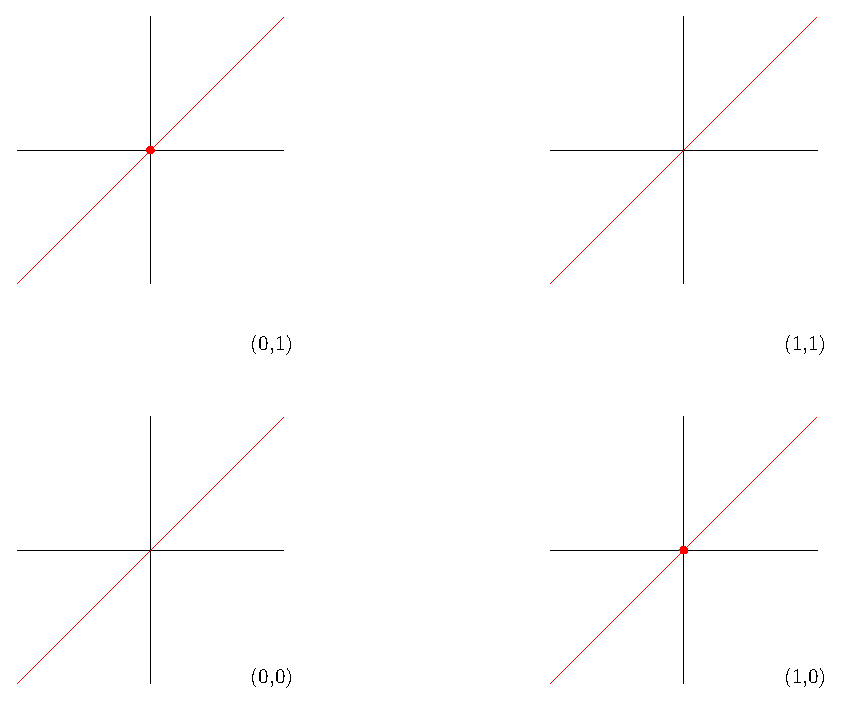
\includegraphics[scale=0.5]{graph.eps}
		\end{minipage}
	\end{example}
	\begin{prop}
		Si $\quot{X}{\sim}$ est séparé, alors le graphe de la relation  $\sim$ est fermé.
	\end{prop}
	Pour arriver à ce résultat nous aurons besoin du Lemme suivant.
	\begin{definition}[Diagonale]
		La diagonale d'un espace X est définie comme le sous ensemble du produit cartésien
	\[\Delta \defeq \{(x,x) \in X \times X\}\]
	\end{definition}
	\begin{lemma}
		\label{lma:diag}
		Un espace est Hausdorff si et seulement si sa diagonale est fermée.
	\end{lemma}
	\begin{proof}
		Soient $x \neq y \in X$ et  $x \in U, y \in V$ des voisinages distincts. Alors  $U\times V$ est un voisinage ouvert de  $(x,y) \in X\times Y$ munit de la topologie produit. On observe que  $U\cap V \neq \varnothing \iff (U\times V) \cap \Delta = \varnothing$. On peut séparer x et y par des ouverts si et seulement si $\Delta^c$ est ouvert.
	\end{proof}
	\begin{proof}[Démonstration de la proposition]
		Si le quotient $\quot{X}{\sim}$ est séparé, la diagonale $\Delta \subset (\quot{X}{\sim})^2$ est fermée par le \textbf{Lemme} \ref{lma:diag}. On considère $q\times q : X \times X \longmapsto (\quot{X}{\sim}) \times (\quot{X}{\sim})$ le quotient et on identifie \[
		{(q \times q)}^{-1}(\Delta) = \{(x,y) \in X \times X \;|\; [x] = [y]\} = \Gamma 
		\] qui est donc fermé.	
	\end{proof}
	Bien que nécessaire, notons que cette condition n'est pas suffisante. Le critère suivant fournit quant à lui une condition suffisante, bien que non nécessaire. 
	\begin{definition}[Saturé]
		On appelle saturé de $A$ l'ensemble $q^{-1}(q(A))$ pour  $A \subset X$.
	\end{definition}

	\begin{prop}
		Si $X$ est un espace séparé tel que $q^{-1}(q(x))$ est compact pour tout  $x\in X$ et $q^{-1}(q(F))$ est fermé dans $X$ pour tout F fermé dans $X$, alors $\quot{X}{\sim} = q(X)$ est séparé
	\end{prop}
	\begin{proof}
		Prenons deux classes disjointes du quotient $[x] \neq [y]$. Puisque $X$ est séparé on peut trouver deux ouverts disjoints de $X$, $U$ et $V$, avec $q^{-1}(x) \in U$ et  $q^{-1}(y) \in V$ puisque $q^{-1}([x])$ et  $q^{-1}([y])$ sont compacts. En regardant les complémentaires fermés on a que \[
			U^c \subset q^{-1}(q(U^c)) \; \text{et} \; V^c \subset q^{-1}(q(V^c))
		.\] Soient donc \[
		U' \defeq X\setminus(q^{-1}(q(U^c))) \subset U \; \text{et} \; V' \defeq X\setminus(q^{-1}(q(V^c))) \subset V
	.\]  On va prouver que $q(U')$ et  $q(V')$ sont des voisinages ouverts et disjoints de $[x]$ et $[y]$ respectivement. 
	D'abord $[x] \in q(U')$ car  $x \not\in q^{-1}(q(U^c))$ et de même  $[y] \in q(V')$. Pour montrer que $q(U')$ est ouvert, on montre que  $U' = q^{-1}(q(U'))$. La première inclusion est toujours vérifiée, montrons la seconde. Soit $u \in q^{-1}(q(U'))$, alors $q(u) \in q(U')$ et donc $q(u) \not\in q(U^c)$. Ainsi  $u \not\in q^{-1}(q(U^c))$, donc $u \in U'$ par construction de $U'$, de même pour $V'$. \\
	Pour terminer la preuve, montrons que $q(U')$ et  $q(V')$ sont disjoints. Supposons par l'absurde que ce ne soit pas le cas. Soit $[z] \in q(U')\cap q(V')$, il existe donc $u' \in U'$ tel que  $[z] = q(u') \in q(V')$. Ainsi $u' \in q^{-1}(q(V')) = V'$ mais  $U'$ et  $V'$ sont disjoints, contradiction.
	\end{proof}
	\begin{cor}
		Si $A \subset X$ est un sous espace compact et $X$ séparé, alors $\quot{X}{A}$ est séparé.
	\end{cor}
	\begin{proof}
		Le critère précédent est vérifié puisque la saturation d'un point
		\begin{align*}
			q^{-1}(q(x)) = \begin{cases}
				A \; \text{si} \; x \in A \\
				\{x\} \; \text{sinon} 
			\end{cases}
		.\end{align*} Dans les deux cas ce sont des compacts.
		Si $F \subset X$ est fermé alors 
		\begin{align*}
			q^{-1}(q(F)) = \begin{cases}
				F \; \text{si} \; A\cap F = \varnothing \\
				F \bigcup A \; \text{sinon}
			\end{cases}
		.\end{align*} Notons que $A$ est fermé puisque compact dans un espace séparé, ce qui implique que  $F \bigcup A$ l'est également.
	\end{proof}
	\begin{example} On montre à travers cet exemple que cette proposition n'est \emph{pas} nécessaire. On définit sur $\mathbf{R}^2$ la relation  \[
		\textbf{x} \sim \textbf{y} \iff \exists \textbf{a} \in \mathbf{Z}^2 \;|\; \textbf{x} + \textbf{a} = \textbf{y}
	.\] Alors $\quot{\mathbf{R}^2}{\sim}$ est compact et séparé mais $q^{-1}(q(\textbf{0})) = \mathbf{Z}^2$ n'est pas compact.
	\end{example}

	\begin{prop}
		L'espace $\quot{X}{\sim}$ est T1, ou de Fréchet, si et seulement si chaque classe d'équivalence de $\sim$ est fermée dans $X$.
	\end{prop}
	
	Dans le cas où $X$ est un espace compact on a des équivalences plus satisfaisantes.
	 \begin{prop}
		Soit $X$ un espace compact, alors $\quot{X}{\sim}$ est séparé si et seulement si le graphe de la relation $\sim$ est fermé.
	\end{prop}

	\begin{definition}[Espace projectif réel]
		Soit $S^n \subset \mathbf{R}^{n+1}$ la sphère unité et $\sim$ la relation définie par $x \sim y \iff x = \pm y$ pour $x,y \in S^n$. L'espace projectif réel $\mathbf{RP}^n$ est le quotient  $\quot{S^n}{\sim}$.
	\end{definition}
	\begin{prop}
		$\mathbf{RP}^n$ est compact et séparé.
	\end{prop}
	\begin{proof}
		$S^n$ est compact le quotient l'est aussi. De plus $q^{-1}(q(x)) = \{\pm x\}$ est compact et $q^{-1}(q(F)) = F \bigcup -F$ est fermé comme union de deux fermés et donc par la proposition précédente le quotient est séparé.
	\end{proof}
	On passe de $\mathbf{R}$ à  $\mathbf{C}$ et on remplace les nombre réels de valeur absolue 1 par  $S^1 \subset \mathbf{C}$ les nombres complexes de module 1.

	\begin{definition}[Espace projectif complexe]
		Soit $S^{2n+1} \subset \mathbf{C}^{n+1}$ la sphère unité et la relation $\sim$ définie par  $x \sim y  \iff x = a\cdot y$ pour un $a \in S^1$. Le quotient $\mathbf{CP}^n$ est l'espace projectif complexe de dimension  $n$.
	\end{definition}

	\section{Quotient par des actions de groupe}

	\begin{definition}[Groupe topologique]
		Un groupe topologique $(G,\star)$ est un groupe munit d'une topologie pour laquelle les applications de multiplication et d'inversion \[
			G^2 \longmapsto G : (x,y) \longmapsto x \star y \qquad \text{et} \qquad G \longmapsto G : x \longmapsto x^{-1}
		\] soient continues. Il est bon de noter qu'ici $G^2$ est munit de ma topologie produit. 
	\end{definition}

	\begin{prop}
		Un groupe $(G,\star)$ munit d'une topologie est un groupe topologique si et seulement si l'application  \[
			G^2 \longmapsto G : (x,y) \longmapsto x \star y^{-1}
		\] est continue. 
	\end{prop}
	Afin d'alléger les notations, dans la suite de cette section lorsque cela ne prête pas à confusion on omettra de noter explicitement la loi de $G$. 

	\begin{example} On donne quelques exemples de base de groupes topologiques
		\begin{enumerate}
			\item Tout groupe munit de la topologie discrète est un groupe topologique, il est parfois noté $G^{\delta}$.
			\item $(\mathbf{R}^n,+)$ est un groupe topologique pour la topologie euclidienne.
			\item $(GL_n(\mathbf{R}),\cdot)$ est un groupe topologique muni de la topologie de sous espace de $M_n(\mathbf{R}) \cong \mathbf{R}^{n^2}$. La multiplication et l'inversion de matrices sont des applications continues. 
		\end{enumerate}	
	\end{example}

	\begin{lemma}
		Tout sous groupe d'un groupe topologique est encore un groupe topologique.
	\end{lemma}

	\begin{definition}
		Une action d'un groupe topologique $G$ à droite sur un espace $X$ est donnée par une application continue
		\begin{align*}
			X \times G &\longmapsto X \\
			(x,g) &\longmapsto x\cdot g
		\end{align*} satisfaisant 

		\begin{enumerate}
			\item $x \cdot 1_G = x$
			\item $x \cdot (gh) = (x \cdot g)\cdot h$
		\end{enumerate}
	\end{definition}

	\begin{definition}[Espace des orbites]
		Soit $X$ un espace sur lequel $G$ agit. L'espace des orbites $\quot{X}{G}$ est le quotient de $X$ par la relation $x \sim y \iff \exists g \in G \;|\; x = y \cdot g$.
	\end{definition}
	\begin{example}
		\begin{enumerate}
			\item Le groupe $C_2$ agit  sur  $S^n \subset \mathbf{R}^{n+1}$ par l'action antipodale, le générateur $g\in C_2$ agit par $x\cdot g = -x$. Alors $\quot{S^n}{C_2} \cong \mathbf{RP}^n$. 
			\item Le groupe $S^1 \defeq \{z\in \mathbf{C} \;|\; |z| = 1\}$ agit par multiplication  à droite sur les coordonnées de $S^{2n+1} \subset \mathbf{C}^{n+1}$. Pour $z\in S^1$ et $a=(a_0,\ldots,a_n) \in S^{2n+1}$, $a\cdot z = (a_0z,\ldots,a_nz)$. Le quotient $\quot{S^{2n+1}}{S^1} \cong \mathbf{CP}^n$. 
			\item Le groupe (discret) $(\mathbf{Z}^2,+)$ agit par translation sur le plan $\mathbf{R}^2$, le quotient $\quot{\mathbf{R}^2}{\mathbf{Z}^2}$ est un tore.
			\item Le groupe $S^1$ agit par rotations d'axe vertical sur $S^2$, les orbites sont les parallèles et les pôles. Le quotient $\quot{S^2}{S^1} \cong I$, les classes des pôles sont les extrémités de l'intervalle.
		\end{enumerate}	
	\end{example}
	\begin{remark}
		Étant donne un groupe $G$ et un sous groupe $H < G$, $H$ agit naturellement sur $G$ par multiplication
		\begin{align*}
			G\times H &\longmapsto G\\
			(g,h) &\longmapsto gh
		.\end{align*}
		L'espace quotient $\quot{G}{H}$ est l'espace des orbites $gH$. En particulier ces dernières ont toutes le même cardinal. Lorsque $H \triangleleft G$, l'espace quotient $\quot{G}{H}$ hérite d'une structure de groupe.
	\end{remark}

	\begin{prop}
		Soit $G$ un groupe topologique agissant sur un espace $X$, alors
		\begin{enumerate}
			\item Le quotient $q : X \longmapsto \quot{X}{G}$ est une application ouverte.
			\item Si $X$ est compact alors le quotient l'est aussi.
			\item Si $X$ et $G$ sont compact et séparés alors le quotient l'est aussi.
		\end{enumerate}
		\begin{proof}
			\begin{enumerate}
				\item Puisque la multiplication par $g$ est un homéomorphisme 
					 \begin{align*}
						 X &\longmapsto X \\
						 x &\longmapsto x\cdot g
					\end{align*}
					si $U \subset X$ est ouvert alors $U \cdot g$ l'est aussi. Pour montrer que $q(U)$ est ouvert dans le quotient on doit montrer par définition de la topologie quotient que la primage est ouverte dans X. Or  $q^{-1}(q(U)) = \bigcup_{g\in G}U\cdot g$, est ouvert comme union d'ouverts.
				\item L'image d'un compact par une fonction continue est compact.
				\item Comme $X$ est séparé, la diagonale $\Delta$ est fermée dans $X \times X$par le \textbf{Lemme} \ref{lma:diag} donc compacte. On pose
					\begin{align*}
						X \times X \times G &\longmapsto X \times X \\
						(x,y,g) &\longmapsto (x,yg)
					.\end{align*}
					L'image de $\Delta \times G$, compact, est le graphe $\Gamma$ de la relation, qui est compact. X étant séparé $\Gamma$ est fermé. Soient  $x,y \in X$ avec $xG \neq yG$. Comme  $(x,y) \not\in \Gamma$, il existe un voisinage dans $X\times X$ de $(x,y)$ disjoint de  $\Gamma$. On peut choisir ce dernier par définition de la topologie produit comme $U\times V$ avec $U,V \subset X$ des ouverts.  \\
					On affirme que les ouverts $q(U)$ et  $q(V)$ (ouverts par le premier point de la proposition) séparent les orbites  $xG$ et $yG$. Si  $zG \in q(U)\cap q(V)$ alors $z = ug_1 = vg_2$ avec $u\in U,v \in V, g_1,g_2\in G$. Mais alors $(u,v) = (u,ug_1g^{-1}_2) \in U\times V \cap \Gamma$, contradiction.
			\end{enumerate}
		\end{proof}
	\end{prop}
	\begin{example}
		$\mathbf{RP}^n$ et $\mathbf{CP}^n$ sont compacts et séparés.
	\end{example}

	\section{Les espaces projectifs}

	\begin{definition}[Stabilisateur]
		Le stabilisateur de $x\in X$ est l'ensemble \[
			G_x \defeq \{g\in G \;|\; g\cdot x = x\} 
		.\] 	
	\end{definition}
	\begin{prop}
		Soit $G$ un groupe topologique compact qui agit à gauche transitivement sur un espace $X$ séparé, alors pour tout point $x\in X$ on a un homéomorphisme  \[
			\quot{G}{G_x} \cong X
		.\] 
	\end{prop}
	\begin{proof}
		On pose l'application 
		\begin{align*}
			\varphi_x : G&\longmapsto X \\
			g &\longmapsto g\cdot x
		.\end{align*}
		Puisque l'action est transitive on obtient que $\varphi_x$ est surjective. De plus $$\varphi_x(g) = \varphi_x(g') \iff g\cdot x = g'\cdot x \iff g^{-1}g' \in G_x$$. Ainsi $\varphi_x$ passe au quotient  $\overline{\varphi_x} : \quot{G}{G_x} \longmapsto X$ et on a vu que cette application est surjective et injective. Puisque $\quot{G}{G_x}$ est compact et X est séparé c'est un homéomorphisme.
	\end{proof}

	\begin{example}
		Pour $ n\ge 2$, le groupe $\mathcal{SO}(n)$ agit transitivement sur $S^{n-1} \subset \mathbf{R}^{n}$ par multiplication matricielle à gauche sur les vecteurs colonnes de norme 1.
		Le stabilisateur de $e_n$ est isomorphe à $\mathcal{SO}(n-1)$. Par abus de notation on considère $\mathcal{SO}(n-1)$ comme un sous groupe de $\mathcal{SO}(n)$. On a $\quot{\mathcal{SO}(n)}{\mathcal{SO}(n-1)} \cong S^{n-1}$.\\
		En petites dimensions on a $\mathcal{SO}(1) = \{(1)\}$. Puis $\mathcal{SO}(2) \cong S^1$, enfin $\quot{\mathcal{SO}(3)}{\mathcal{SO}(2)} \cong S^2$.
	\end{example}
	\begin{remark}
$\mathbf{RP}^0 \cong \quot{\{\pm 1\}}{-1 \sim 1}$, $\mathbf{RP}^1 \cong S^1$, $\mathbf{RP}^2 \cong \quot{D^2}{\sim}$
	\end{remark}
	\begin{prop}
		On a un homéomorphisme $\mathcal{RP}^3 \cong \mathcal{SO}(3)$.
	\end{prop}

	\section{Recoller des espaces}
	Soient $f : A \longmapsto X$ et $g : A \longmapsto Y$ deux applications continues. On aimerait construire un nouvel espace à partir de $X$ et $Y$ en identifiant leur `partie commune' $A$.

	\begin{definition}[Recollement]
		Le recollement $X \bigcup_A Y$ est l'espace quotient $\quot{X \coprod Y}{\sim}$ où $\sim$ est la relation d'équivalence engendrée par  $f(a) \sim g(a) \; \forall a \in A$, autrement dit la relation d'équivalence la plus fine avec cette propriété. On appelle cet espace le \textbf{pushout} de $X$ et $Y$.	
	\end{definition}
	\begin{remark}
		Pour les applications suivantes le diagramme de droite commute. \\
		\begin{minipage}{0.5\textwidth}
			\begin{align*}
				&i : X \xmapsto{i_1} X \coprod Y \xmapsto{q} X \bigcup_A Y \\
				& j : Y \xmapsto{i_2} X \coprod Y \xmapsto{q} X \bigcup_A Y			
			\end{align*}
		\end{minipage}
		\hfill
		\begin{minipage}{0.5\textwidth}
			\centering
			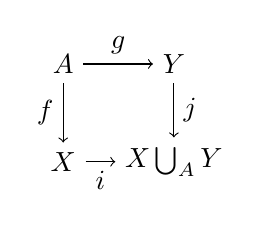
\begin{tikzpicture}[every node/.style={midway}]
				  \matrix[column sep={4em,between origins}, row sep={2em}] at (0,0) {
				    \node(A) {$A$}  ; & \node(Y) {$Y$}; \\
				    \node(X) {$X$}; & \node (U) {$X\bigcup_A Y$};\\
				  };
				  \draw[<-] (X) -- (A) node[anchor=east]  {$f$};
				  \draw[->] (A) -- (Y) node[anchor=south] {$g$};
				  \draw[->] (Y) -- (U) node[anchor=west] {$j$};
				  \draw[->] (X) --(U) node[anchor=north] {$i$};
			\end{tikzpicture}
		\end{minipage}
	\end{remark}
	\begin{prop}[Propriété universelle]
		Pour toutes applications $\alpha : X \longmapsto Z$ et\\
		$\beta : Y \longmapsto Z$ telles que $\alpha \circ f = \beta \circ g$ il existe une \emph{unique} application  $\gamma : X \bigcup_A Y \longmapsto Z$ telle que $\gamma \circ i = \alpha$ et  $\gamma \circ j = \beta$.

		\begin{minipage}{0.5\textwidth}
			Le diagramme suivant résume cette propriété, $\gamma$ est l'unique application le faisant commuter.
		\end{minipage}
		\hfill
		\begin{minipage}{0.5\textwidth}
			\[
			\xymatrix@R=1.2cm@C=1.2cm{
			 A \ar[r]^{g}      \ar[d]_{f}         & Y \ar[d]_{j} \ar@/^1pc/[rdd]^{\beta}   \\
			 X \ar[r]^{i} \ar@/_1pc/[rrd]_{\alpha} & X\bigcup_A Y \ar@{-->}[rd]|{\exists! \; \gamma}             \\
							      &                                   & Z 
			}
	\]	
		\end{minipage}
	\end{prop}
	\begin{proof}
		Pour définir $\gamma$ on pose  
		\begin{align*}
			H : X \coprod Y &\longmapsto Z \\
			x &\longmapsto \alpha(x) \\
			y &\longmapsto \beta(x)
		.\end{align*}
		Ce choix passe au quotient car $H(f(a)) = \alpha(f(a)) = \beta(g(a)) = H(g(a))$. On pose  $\gamma \defeq \overline{H}$ l'unicité est quant à elle claire.
	\end{proof}
	
	\begin{figure}[ht]
		\centering
		\def\svgwidth{0.5\textwidth}
		\input{pushout.pdf_tex}
		\caption{Illustration du pushout de $X$, $Y$ par leur `partie commune' $A$.}
	\end{figure}

	\begin{lemma}
		\label{lma:2}
		Soient $X,Y$ des espaces séparés, $A\subset Y$ fermé, $f : A \longmapsto X$ continue. Si $C \subset X$, alors $q^{-1}(q(C)) = C \amalg f^{-1}(C)$. 
	\end{lemma}
	\begin{lemma}
		\label{lma:3}
		Soient $X,Y$ des espaces séparés,  $A\subset Y$ fermé. Si $C \subset Y$, alors \[q^{-1}(q(C)) = f(A\cap C) \amalg (C \cup f^{-1}(f(A\cap C))).\]
	\end{lemma}
	\begin{proof}
		Soit $y \in C$. Si $y\in C \setminus A, \; [y] = \{y\}$. Sinon $[y] = f(y) \amalg f^{-1}(f(y))$. Donc $q^{-1}(q(C)) = (C\setminus A) \cup (C \cap A) \cup f(C\cap A) \cup f^{-1}(f(C\cap A))$ 	
	\end{proof}
	\begin{prop}
		Soient $X,Y$ des espaces séparés,  $A\subset Y$ compact, alors $X \cup_A Y$ est séparé.
	\end{prop}
	\begin{proof}
		On vérifie le critère de séparation. Les deux lemmes nous permettent de décrire la saturation d'un fermé arbitraire de $X \coprod Y$. Un fermé de  $X \coprod Y$ est une réunion disjointe de fermés, il suffit donc de vérifier ce qui se passe pour $C \subset X$ fermé et pour $C$ fermé de  $Y$.\\ 
		Dans le premier cas, le \textbf{Lemme} \ref{lma:2} montre que $q^{-1}(q(C)) = C \amalg f^{-1}(C)$ est fermé. \\
		Dans le second le \textbf{Lemme} \ref{lma:3} montre que $q^{-1}(q(C)) =f(C\cap A) \amalg f^{-1}(f(A\cap C))$. Ici $C\cap A$ est fermé dans $A$, donc compact. L'image par $f$ est donc un compact dans $X$ qui est séparé, elle est donc fermée. On conclut ensuite que $f^{-1}(f(A\cap C))$ est fermé aussi. \\ 
	On vérifie finalement que la saturation d'un point est compacte, par exemple si \[y \in A, \; q^{-1}(q(y)) = f(y) \amalg f^{-1}(f(y))\] qui est une union disjointe de compacts donc un compact.
	\end{proof}
	
	\begin{cor}
		Soit $X$ un espace séparé, $A$ compact et séparé, $f : A\longmapsto X$. Alors $X \cup_f CA$ est séparé et compact si $X$ est compact.
	\end{cor}
	\begin{proof}
		Comme $A$ est séparé, $CA$ est séparé, on applique la \textbf{Proposition 1.6.5}.
	\end{proof}

	Un cas particulier et important de la construction du pushout $X \cup_A Y$ est celui où $g : A \hookrightarrow CA$ est l'inclusion de la base du cône. 
	\begin{definition}[Attachement de cellule]
		Étant donné une application $f : A \longmapsto X$ on dit que le pushout $X \cup_A CA$ aussi noté $X \cup_f CA$ est obtenu de X en attachant une $A-$\textit{cellule} le long de $X$. \\
		Lorsque $A = S^{n-1}$ on dit que $X \cup_f e^n$ est obtenu en attachant une $n-$\textit{cellule} le long de $f$. \\
		L'application $f$ est appelée \textit{application d'attachement}.
	\end{definition}

	\begin{prop}
		Soient $f,f' : A \longmapsto X$ homotopes. Alors \[
			X \cup_f CA \simeq X \cup_{f'} CA
		.\] 
	\end{prop}
	\begin{proof}
		On doit trouver deux applications
		\begin{align*}
			&h : Y \longmapsto Y' \\
			&h' : Y' \longmapsto Y
		\end{align*}
		telles que $h\circ h' \simeq id_Y$ et $h'\circ h \simeq id_{Y'}$. 
		On construit $h$ par passage au quotient d'une application 
		 \begin{align*}
			 X \amalg CA &\longmapsto Y' \\
				 x&\longmapsto x \\
				 [a,t]& \longmapsto \begin{cases}
					 [a,2(t-\frac{1}{2})] \; &\text{si} \; \frac{1}{2} \le t \le 1 \\
					 H(a,2t) \; &\text{si} \; 0 \le t \le \frac{1}{2}
			 \end{cases}
		\end{align*}
		où $H : A \times I \longmapsto X$ est une homotopie de $f \longmapsto f'$.
		La moitié supérieure du cône $CA$ dans $Y$ est envoyée sur \emph{tout} le cône de $Y$. On vérifie que pour $t=\frac{1}{2}$, \[[a,2(t-\frac{1}{2})] = [a,0] = [f'(a)] = [H(a,1)] = [H(a,2\cdot \frac{1}{2})].\]
		Pour $t=0$, $H(a,0) = f(a)$ si bien qu'elle passe au quotient. On procède de même pour $h'$ avec $H(\cdot , 1-t)$, homotopie de  $f' \longmapsto f$. \\
		Calculons $h' \circ h$. On observe que $(h'\circ h)|_X$ est l'identité, puis que sur $CA$ on a \[
			(h'\circ h)[a,t] = \begin{cases}
				[a,2t-1] \xmapsto{h'} [a,4t-3] \; &\text{si} \; \frac{3}{4} \le t \le 1 \\
				[a,2t-1] \xmapsto{h'} H(a,3-4t) \; &\text{si} \; \frac{1}{2} \le t \le \frac{3}{4} \\
				H(a,2t) \xmapsto{h'} H(a,2t) \; &\text{si} \; 0 \le t \le \frac{1}{2}
			\end{cases}
		.\] 
		On parcourt le cône $CA$ de $Y$ quatre fois plus rapidement sur le quart supérieur, ensuite on utilise $H$ pour faire le lien entre $f$ et $f'$, puis on revient en arrière avec l'homotopie inverse. \\
		On doit enfin construire une homotopie \[
			h'\circ h \times I \longmapsto id_{Y}
		.\] 
		L'idée est de définir $K : Y \times I \longmapsto Y$ de sorte qu'au temps $s$ on commence par l'homotopie $H$ mais seulement jusqu'au temps $t=s$, puis on revient en arrière et on termine avec l'identité.
		On pose $K|_{X\times I}$ comme étant la projection sur $X$ puis on pose  \[
			K([a,t],s) = \begin{cases}
				[a, \frac{4}{4-3s}t-\frac{3s}{4-3s}] \; &\text{si} \; \frac{3}{4}s \le t \le 1 \\
				H(a,3s-4t) \; &\text{si} \; \frac{s}{2} \le t \le \frac{3}{4}s \\
				H(a,2t) \; &\text{si} \; 0 \le t \le \frac{s}{2}
			\end{cases}
		.\] 
		On vérifie que 
		\begin{align*}
			K([a,t],0) = [a,t] = id_{CA}[a,t] \\
			K([a,t],1) = (h'\circ h)([a,t])
		.\end{align*}
		De même on définit $K'$ une homotopie de $id_{Y'} \longmapsto h \circ h'$.
	\end{proof}
	\begin{cor}
		Si $f \simeq f' : S^{n-1} \longmapsto X$, alors $X \cup_f e^n \cong X \cup_{f'}e^n$. En particulier si $f$ est homotope à une fonction constante, alors $X \cup_f e^n \cong X \bigvee S^n$.
	\end{cor}
	\begin{prop}
		$D^n \cong CS^{n-1}$.
	\end{prop}
	\begin{example}
		Le même espace topologique peut admettre des descriptions distinctes comme recollement de cellules. Par exemple $S^1 \cong \star \cup e^1$ où  $f : S^0 \longmapsto \star$ est constante, mais on a aussi $S^1 \cong S^0 \cup_f e^1 \cup_g e'^1$. La deuxième description est compatible avec l'action antipodale de $C_2$ tandis que la première ne l'est pas, au sens que si $g$ engendre  $C_2$,  $g \cdot g$ transforme une cellule en cellule, si bien que $\mathbf{RP}^1 \cong \star \cup e^1 \cong S^1$.
	\end{example}

	\section{Quelques surfaces}
	\begin{definition}[Surface]
		Une surface est un espace séparé où tout point admet un voisinage ouvert homéomorphe à un disque ouvert.	
	\end{definition}
	\begin{example}
		$S^2, T^2, \mathbf{RP}^2, K$ sont des surfaces. 
	\end{example}
	\begin{definition}[Somme connexe]
		La somme connexe $S\#T$ de deux surfaces $S$ et $T$ est obtenue en choisissant deux points $s \in S, t \in T$ puis deux ouverts contenant chacun un de ces points $U, V \cong D^2, \; s \in U, t \in V$ et en construisant le quotient \[
			\quot{(S\setminus U)\coprod (T \setminus V)}{x\sim f(x)}
		\] 
			où $f : \partial U \xmapsto{\cong} S^1 \xmapsto{\cong} \partial V$.
	\end{definition}
	On peut construire de nouvelles surfaces à l'aide de vielles surfaces grâce à l'opération de somme connexe.
	\begin{example}
		$S\#S^2 \cong S$ par le théorème du disque de Palais (1960), cette construction est bien définie à homéomorphisme près.
	\end{example}
	\begin{example}
		$T^2\#T^2$ est homéomorphe à un tore à deux trous.
	\end{example}
	\begin{figure}[ht]
			\centering
			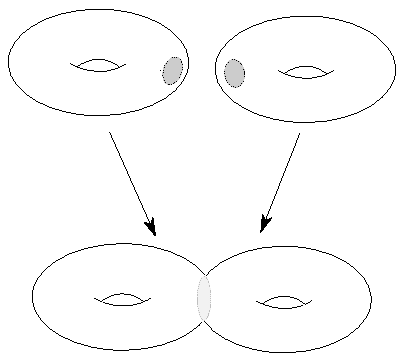
\includegraphics{connectedsum.pdf}
			\caption{Illustration de la somme connexe de deux 2-Tores.}
	\end{figure}
\end{document}
